\documentclass[10pt,a4paper]{article}
\usepackage{fontspec,amsmath,amssymb,amsthm,mathtools,graphicx,bm,bbm,stmaryrd,nicefrac,mathrsfs,braket}
\usepackage[margin=22mm]{geometry}
\usepackage[bookmarks=false]{hyperref}
\setlength{\emergencystretch}{3em}
\title{Maximal randomized versus pseudo-deterministic quantum query separation}
\author{Hugo Aaronson, Tom Gur, Jiawei Li}
\date{doi:10.4230/LIPIcs.ICALP.2026.3; CC BY 4.0}
\begin{document}
\maketitle
\noindent\textit{Editorial note.} Editable TeX converted from the official CC BY HTML prose and math alttext. Original official PDF/HTML retained. Only the specified claim counts; all author context and available source-local supporting proofs are included. Theorems 5, 6, 7 and quantum-input extensions whose proofs are deferred to a full version are retained only as author context and are not collected proof claims.\par\medskip


\par\medskip\noindent\textbf{
1 Introduction}\par




The study of pseudo-deterministic algorithms, initiated by Gat and Goldwasser [13], is concerned with randomized algorithms that output a canonical solution for each input. That is, a randomized algorithm $\mathcal{A}$ that solves a search problem ${R}\subseteq\mathcal{X}\times\mathcal{Y}$ is said to be pseudo-deterministic if there exists a function $f:\mathcal{X}\rightarrow\mathcal{Y}$ such that for any input $X\in\mathcal{X}$, the output $\mathcal{A}(X)$ is $f(X)$ with high probability.\par




Pseudo-deterministic algorithms capitalize on the computational power of randomization while still maintaining the predictable output behaviour of deterministic algorithms. This stands in contrast to fully randomized algorithms, whose repeated runs may return vastly different outputs.
Over the last decade, pseudo-deterministic algorithms have received much attention and have appeared across diverse areas of theoretical computer science [15, 16, 14, 17, 10, 11, 7, 8, 6, 19].\par




In the quantum setting, pseudo-deterministic algorithms were first considered by Goldwasser, Impagliazzo, Pitassi and Santhanam [18] when studying the Find1 problem\footnote{The input to the Find1 problem is a string $X\in\{0,1\}^{N}$ with the promise that $X$ has Hamming weight at least $N/2$, and the goal is to output an index $i$ with $X_{i}=1$.}
for pseudo-deterministic algorithms in the query complexity model. While Find1 is solvable in $O(1)$ queries by random sampling, they showed that any pseudo-deterministic algorithm, classical or quantum, for Find1 requires ${\Omega}(\sqrt{N})$ queries.\par




What makes quantum pseudo-determinism truly distinct is the randomness that arises from \emph{measurement}.
Many quantum algorithms that achieve exponential quantum speed-up (e.g., Fourier sampling) measure superpositions over exponentially many candidate solutions, a step that appears inherent. This offers a new perspective to revisit existing quantum advantages:\par





{\itshape When can quantum speed-ups be achieved pseudo-deterministically,

and when does quantum advantage inherently require output entropy?}\par





This question also links quantum pseudo-determinism to certified randomness: if one can show that the quantum advantages of a certain problem ${R}$ cannot be preserved given the pseudo-deterministic requirement, then any (potentially untrusted) quantum device $\mathcal{A}$ that solves ${R}$ efficiently must generate some entropy.
A series of works [4, 3, 23] show, under standard complexity assumptions, that Fourier sampling [1], random-circuit sampling, and the Yamakawa–Zhandry algorithm [23] cannot be made pseudo-deterministic\footnote{For quantum certified randomness, these works in fact prove quantitatively stronger statements: any efficient quantum algorithm for these tasks must generate a large amount of min-entropy.}.\par




Motivated by the above, we initiate a systematic study of quantum pseudo-determinism. We investigate the fundamental properties of pseudo-deterministic quantum algorithms, show complexity separations that shed light on the strength and limitations of quantum pseudo-determinism, and identify a wide class of problems (which includes Grover search, element distinctness, triangle finding, $k$-sum, and graph collision) that admit efficient pseudo-deterministic quantum algorithms.\par




\par\medskip\noindent\textbf{
1.1 Our results}\par




We start with the query complexity model. Unless otherwise stated, we denote the length of the input to the search problem by $N$. For a search problem ${R}$, we denote the deterministic query complexity by $\mathsf{D}({R})$, the pseudo-deterministic quantum query complexity $\mathsf{psQ}({R})$, and the quantum query complexity by $\mathsf{Q}({R})$. We denote the output of algorithm $\mathcal{A}$ given query access to input $X$ as $\mathcal{A}^{X}$.\par




\par\medskip\noindent\textbf{
1.1.1 Query complexity separations}\par




We first study the relationship between pseudo-deterministic quantum query algorithms, randomized algorithms, and classical pseudo-deterministic algorithms.\par




\par\medskip\noindent\textbf{Hardness of quantum pseudo-determinism}\par




Our first result shows that not all problems admit efficient pseudo-deterministic quantum algorithms. We give a maximal separation between classical randomized query complexity and quantum pseudo-deterministic query complexity.\par




% SOURCE-ID Thmtheorem1


\par\medskip\noindent\textbf{
\textbf{Theorem 1}\textbf{.}
}\par



\emph{There exists a search problem ${R}$ whose classical randomized complexity is $O(1)$ and whose pseudo-deterministic quantum query complexity is $\Omega(N)$.}\par



% END-SOURCE-ID Thmtheorem1




Theorem 1 improves the separation given by the Find1 problem, where the pseudo-deterministic quantum lower bound is $\Omega(\sqrt{N})$.
We obtain this stronger separation via the \emph{Avoid One Encrypted String} (AOES) problem. Informally, the input encodes $m$ instances of XOR gadgets; together they encrypt a hidden string $b\in\{0,1\}^{m}$, where $b_{i}$ is the solution to the $i$-th XOR instance. The goal is to output any $m$-bit string \emph{not equal} to $b$. A classical randomized algorithm succeeds with constant probability by blind sampling, whereas any pseudo-deterministic algorithm must consistently avoid $b$ across runs, effectively forcing it to learn at least one bit of $b$.\par





\par\medskip\noindent\textbf{Power of quantum pseudo-determinism}\par




Our second result shows that pseudo-deterministic quantum algorithms can be much stronger than their classical counterparts. We prove an exponential separation between pseudo-deterministic quantum algorithms and pseudo-deterministic classical algorithms on a task that remains easy for classical randomized algorithms. To ensure this separation is meaningful, we need to be certain that the quantum algorithm is not simply introducing solutions inaccessible to classical computation. We do this by defining the notion of “canonization”. Intuitively, this is where a quantum algorithm stabilizes a solution that occurs with considerable probability in a randomized algorithm into a canonical solution, thus canonizing it from a randomized solution to a pseudo-deterministic one.\par



% SOURCE-ID Thmtheorem2


\par\medskip\noindent\textbf{
\textbf{Definition 2}\textbf{.}
}\par



\emph{Let ${R}\subseteq\mathcal{X}\times\mathcal{Y}$ be a search problem with randomized algorithm $\mathcal{A}$ and let $f:\mathcal{X}\rightarrow\mathcal{Y}$ be a function. $f$ canonizes $\mathcal{A}$ if, for any $X\in\mathcal{X}$, the probability $\mathcal{A}^{X}$ outputs $f(X)$ is greater than the probability it outputs an incorrect solution. Equivalently,}\par


\[\begin{gathered}
\forall X\in\mathcal{X}:\mathbb{P}_{\mathcal{A}}[\mathcal{A}^{X}=f(X)]>\mathbb{P}_{\mathcal{A}}[(X,\mathcal{A}^{X})\not\in{R}].
\end{gathered}\]


\emph{A pseudo-deterministic algorithm $\mathcal{B}$ canonizes $\mathcal{A}$ if the function $f$ calculated by $\mathcal{B}$ canonizes $\mathcal{A}$.}\par



% END-SOURCE-ID Thmtheorem2



We now state the theorem that demonstrates the quantum advantage on pseudo-deterministic algorithms.\par



% SOURCE-ID Thmtheorem3


\par\medskip\noindent\textbf{
\textbf{Theorem 3}\textbf{.}
}\par



\emph{There exists a search problem ${R}$ such that}\par


\begin{enumerate}


\item[] 
1. 


\emph{there exists a randomized classical algorithm }$\mathcal{A}$\emph{ for }${R}$\emph{ that uses }$O(\log N)$\emph{ queries;}\par





\item[] 
2. 


\emph{there exists a quantum pseudo-deterministic algorithm }$\mathcal{B}$\emph{ with }$O(\log N)$\emph{ query complexity that canonizes }$\mathcal{A}$\emph{;}\par





\item[] 
3. 


\emph{any classical pseudo-deterministic algorithm for }${R}$\emph{ requires }$\Omega(\sqrt{N})$\emph{ queries.}\par





\end{enumerate}



% END-SOURCE-ID Thmtheorem3



We make two remarks about the conditions required for showing a conceptually meaningful quantum advantage in the setting of pseudo-deterministic algorithms. First, note that without requiring the problem to be easy for randomized algorithms (Item 1), such a separation would be trivial, in the sense that it need not refer to pseudo-determinism at all (e.g., by Simon’s problem, which has a unique solution). In contrast, Theorem 3 exhibits a different form of quantum advantage: beyond faster search, quantum algorithms can \emph{break symmetry} (by eliminating output randomness) more efficiently than classical pseudo-deterministic algorithms.
Furthermore, we also require that such a quantum pseudo-deterministic algorithm canonizes a classical one. This is because we do not want the quantum algorithm to \emph{cheat} by outputting a new solution that is inaccessible to classical algorithms.\par






\par\medskip\noindent\textbf{
1.1.2 Fundamental properties of quantum pseudo-determinism}\par




Next, we provide theorems that demonstrate two basic properties of pseudo-deterministic quantum algorithms: a limitation on maximal speed-ups for total problems, and a general pseudo-deterministic quantum query upper bound via the completeness of the Find1 problem.\par




\par\medskip\noindent\textbf{Deterministic emulation of total problem}\par




We show that for total problems, pseudo-deterministic quantum algorithms cannot exhibit exponential speed-up over classical algorithms. In particular, pseudo-deterministic quantum algorithms for total problems can be emulated by deterministic algorithms with a quintic blow-up.\par



% SOURCE-ID Thmtheorem4


\par\medskip\noindent\textbf{
\textbf{Theorem 4}\textbf{.}
}\par



\emph{Let ${R}\subseteq\{0,1\}^{N}\times\mathcal{Y}$ be a total search problem, then the following holds.}\par




$\mathsf{D}(R)=O(\mathsf{psQ}(R)^{5}\log(N))$\emph{.}\par



% END-SOURCE-ID Thmtheorem4



In contrast, in the classical setting, it was shown in [15] that pseudo-deterministic classical algorithms for total problems can be emulated by deterministic algorithms with a quartic blow-up $\mathsf{D}(R)=O(\mathsf{psR}(R)^{4}\log(N))$. Our proof of Theorem 4 follows the strategy of [15], but poses a new challenge; namely, our main technical contribution in the proof of Theorem 4 is a lemma (Lemma 19) that upper bounds the number of possible outputs of a pseudo-deterministic quantum algorithm; this step is trivial in the classical case.\par





\par\medskip\noindent\textbf{General pseudo-deterministic quantum query upper bound}\par




We also observe that the completeness result in [18], which states that the Find1 problem is \emph{complete} for pseudo-deterministic classical query complexity, extends to the quantum setting. By combining it with the fact that $\mathsf{psQ}({\text{Find1}})=\Theta(\sqrt{N})$ [18],\footnote{An $\tilde{O}(\sqrt{N})$ upper bound for Find1 is informally given in [18]. We make a more careful analysis and show that this logarithmic term can be avoided. See the full version of this paper for details.} we derive a general upper bound on the pseudo-deterministic quantum query complexity of any problem via its randomized query complexity and verification complexity (i.e., the deterministic query complexity of verifying whether an input-solution pair is in a relation).\par



% SOURCE-ID Thmtheorem5


\par\medskip\noindent\textbf{
\textbf{Theorem 5}\textbf{.}
}\par



\emph{For any search problem ${R}$ with randomized query complexity $\mathsf{R}(R)$ and verification complexity $\mathsf{V}(R)$, we have $\mathsf{psQ}(R)=O\big((\mathsf{R}(R)+\mathsf{V}(R))\cdot\sqrt{N}\big)$.}\par



% END-SOURCE-ID Thmtheorem5



This implies that any lower bound for a pseudo-deterministic quantum query complexity problem greater than $\Omega(\sqrt{N})$ requires either a high randomized query complexity or it is difficult to verify. For instance, in our maximally pseudo-deterministically hard problem AOES (Definition 22), the randomized query complexity is $O(1)$, but it is very hard to verify.\par






\par\medskip\noindent\textbf{
1.1.3 Making quantum algorithms pseudo-deterministic}\par




In [20], it was observed that by integrating Grover’s algorithm in a binary search, one can obtain a pseudo-deterministic quantum algorithm for Find1 that returns the first non-zero index in $\Theta(\sqrt{N})$ queries.\par




We extend this idea further and generalize it to obtain pseudo-deterministic quantum algorithms for a broad family of \emph{$k$-subset finding} problems [9]. Here the input $X\in\Sigma^{N}$ consists of $N$ elements, and the goal is to find a subset of $k$ elements satisfying a predicate. To make the binary-search approach applicable, we introduce a mild condition, Prunable, which informally requires that restricting the search domain does not increase the query cost. We show that for Prunable problems, any subset-finding quantum algorithm can be turned pseudo-deterministic with only a near-linear dependence on $k$.\par



% SOURCE-ID Thmtheorem6


\par\medskip\noindent\textbf{
\textbf{Theorem 6}\textbf{.}
}\par



\emph{Let ${R}$ be a $k$-subset finding problem. If ${R}$ is Prunable, then $\mathsf{psQ}({R})=\tilde{O}(k\cdot\mathsf{Q}({R}))$.}\par



% END-SOURCE-ID Thmtheorem6



We note that many natural $k$-subset finding tasks are Prunable, e.g., $k$-distinctness, triangle finding, and $k$-sum. However, we observe that the condition can fail for $k$-subset finding problems with global structure, such as Find1, when interpreted as a $1$-subset finding problem.\par





\par\medskip\noindent\textbf{
1.1.4 Beyond the query complexity model}\par




Finally, we study pseudo-deterministic quantum algorithms outside the setting of the standard query complexity model; namely, by considering search problems with quantum inputs, as well as the white-box setting.\par




\par\medskip\noindent\textbf{Search problems with quantum inputs}\par




We consider a different sort of search problems for which the input is a quantum state. Here, the query complexity is defined as the number of copies of the input state required to solve the problem.
Pseudo-determinism could be useful in problems such as finding a computational basis element in the support of the input state, finding a state orthogonal to the input state, etc. We show, however, there can be no pseudo-deterministic algorithms if the input domain is a connected continuous space.\par




Nevertheless, we consider a quantum version of Find1 we call Uniform-Support-Finding: finding a computational basis element in the support of an input state $\ket{\psi}$, where $\ket{\psi}$ is promised to be a \emph{uniform} superposition over a subset of basis. We prove that the query complexity of Uniform-Support-Finding is $\Theta(d)$, where $d$ is the dimension of $\ket{\psi}$ (See the full version for details).\par





\par\medskip\noindent\textbf{The white-box setting}\par




Finally, we give the characterization of problems that admit efficient pseudo-deterministic quantum algorithms in the white-box (Turing machine) setting.\par



% SOURCE-ID Thmtheorem7


\par\medskip\noindent\textbf{
\textbf{Theorem 7}\textbf{.}
}\par



\emph{A search problem ${R}$ has a pseudo-deterministic quantum polynomial-time algorithm if and only if ${R}$ is P-reducible\footnote{A P-reduction refers to a deterministic polynomial time Turing reduction.} to some decision problem in BQP.}\par



% END-SOURCE-ID Thmtheorem7



We prove Theorem 7 in the full version of this paper, which is generalized from its classical analog in [15]. Intuitively, Theorem 7 says that any search problem $R$ that has an efficient pseudo-deterministic quantum algorithm if and only if it has a \emph{search-to-decision} reduction to BQP. In other words, any (super-polynomial) pseudo-deterministic quantum advantage for a search problem essentially comes from the quantum advantages for a certain decision problem.\par







\par\medskip\noindent\textbf{
1.2 Techniques}\par




In this section, we provide a taste of our techniques for establishing the query complexity separations in Theorem 1 and Theorem 3. In both cases, the key part is proving query complexity lower bounds for pseudo-deterministic quantum or classical algorithms, where new techniques are needed. This can be attributed to a lack of tools for proving pseudo-deterministic lower bounds, and that well-established techniques such as the polynomial method cannot be directly applied.\par




\par\medskip\noindent\textbf{A maximal separation between randomized and pseudo-deterministic quantum algorithms}\par




A quintessential advantage of randomized algorithms compared to pseudo-deterministic ones is their ability to output random strings.
We consider the following problem, called \emph{Avoid One Encrypted String} (AOES), which capitalizes on this advantage. The input of AOES consists of $m$ instances of the XOR problem in parallel, where $m$ is a big constant. Let $N$ be the total input length and $N/m$ be the input length of each XOR instance. These XOR instances encode a secret string $b\in\{0,1\}^{m}$, where $b_{i}$ is the value of the $i$-th XOR instance. The goal is to output any $m$-bit string that is not equal to $b$.\par




AOES can be solved trivially by randomly sampling an $m$-bit string with accuracy $1-1/2^{m}$. However, it is not difficult to show that no deterministic algorithm can do better than using $N/m$ queries to solve the first XOR instance, and then output any string with the first bit unmatched.
Intuitively, any pseudo-deterministic algorithm that can avoid outputting $b$ consistently must have learned some information about those XOR instances. On the other hand, XOR is maximally hard for quantum query algorithm, i.e., any quantum query algorithm for XOR of length $n$ cannot do any better than a random guess with less than $n/2$ queries [12, 5].\par




To turn the intuitions to a proof, we provide a new \emph{randomized} reduction from XOR to AOES. Namely, we show that if there exists a zero-error quantum algorithm $\mathcal{B}$ for ${\text{AOES}}_{N,m}$ with query complexity $q$, then there exists a quantum algorithm $\mathcal{A}$ for ${\text{XOR}}_{N/m}$ which calls $\mathcal{B}$ once such that for every input $X\in\{0,1\}^{N/m}$,\par


\[\begin{gathered}
\mathbb{P}\left[\mathcal{A}^{X}=\mathsf{XOR}(X)\right]\geq\frac{1}{2}+\frac{1}{2^{m+1}}.
\end{gathered}\]




To prove that, let $\mathcal{B}$ be a solver for the AOES problem, and let $X\in\{0,1\}^{N/m}$ be the XOR instance we want to solve. We build a random AOES instance $Z=(Z_{1},\ldots,Z_{m})$ in two steps. First, we generate $m$ uniformly random string $Y_{1},\ldots,Y_{m}\in\{0,1\}^{N/m}$. Then, for each position $i\in[m]$, we take $Z_{i}=Y_{i}$ with probability $1/2$, and $Z_{i}=Y_{i}\oplus X$ with probability $1/2$.\par




At a high-level, $Y_{1},\ldots,Y_{m}$ can be viewed as a one-time pad, and $X$ is embedded into a random subset of positions in the AOES instance $Z$. The crucial observation is that from the AOES solver $\mathcal{B}$’s perspective, $Z$ is uniformly random, and it has no information about $X$, and where $X$ is embedded in $Z$.
We can show that when we embed $X$ into a certain subset of positions in $Z$ that depends on $\mathcal{B}$, we can then recover the solution of the XOR instance $X$ with certainty. When $\mathcal{B}$ is a zero-error algorithm for AOES, the overall success rate of our randomized reduction is $1/2+1/2^{m+1}$, and any value strictly greater than $1/2$ suffices given the hardness of XOR.\par




Finally, for any pseudo-deterministic algorithm $\mathcal{B}$ for AOES, we can decrease its error rate to $1/2^{2m}$ via $O(m)$ repetitions and picking the most common outputs. We can then plug this extremely low error AOES algorithm into the randomized reduction and still get non-zero advantages on XOR. Note that while the random sampling algorithm has an error rate of $1/2^{m}$, it cannot further reduce it via repetition.\par





\par\medskip\noindent\textbf{Exponential pseudo-deterministic quantum advantage}\par




We construct a problem called Quantum-Locked Estimation (QL-Estimation), which is easy for randomized algorithms as well as quantum pseudo-deterministic algorithms, but is hard for classical pseudo-deterministic algorithms.\par




Let $N=2^{n}$. For simplicity, we sometimes interpret a value $x\in[N]$ as an $n$-bit string in the natural way, and vice versa.
Recall that in Simon’s problem [22],
the input is a function $f:[N]\rightarrow[N]$ which is promised to encode a secret string $s$ such that $f(x)=f(y)\iff(x=y)\vee(x=y\oplus s)$. In the Hamming problem, an input string $X\in\{0,1\}^{N}$ is given, and the goal is to output an estimate of the Hamming weight of $X$ up to additive error $N/10$.\par




In the QL-Estimation problem, the input is simply a pair $(f,X)$, where $f$ is an instance of the Simon’s problem and $X$ is an instance of the Hamming problem.
It is promised that $f$ encodes some string $s$ that is promised to be a valid estimate of the Hamming weight of $X$ ($\big|s-\|X\|_{\mathsf{hw}}\big|\leq 0.09\cdot N$).
The goal is to output an estimate for the Hamming weight of $X$ with an additive error up to $N/10$.\par




The classical randomized algorithm can estimate the Hamming weight with $O(1)$ queries, and a quantum algorithm can calculate the secret string $s$, which is a valid solution by the promise of the problem. Indeed, this quantum algorithm \emph{canonizes} the particular estimate $s$, which is one of the many different estimates of the Hamming weight that a classical randomized algorithm could reasonably produce.\footnote{To ensure the condition of the canonization (Definition 2) is satisfied, we need a slightly adjusted classical random sampling algorithm with $O(\log N)$ queries. See Section 4.2 for more details.}
We view this as a “lock-and-key” construction, where
the Hamming problem locks a canonical solution that is hidden from pseudo-deterministic classical algorithms, while the key is Simon’s problem, to which only quantum algorithms have access.\par




For the lower bound of pseudo-deterministic classical algorithms,
it is helpful to first revisit the pseudo-deterministic hardness of Hamming via a \emph{sensitivity argument}. Suppose for some string $X$ (where $\|X\|_{\mathsf{hw}}=N/2$), the pseudo-deterministic output of some algorithm is $t$. Let $X^{\prime}$ be the string with the smallest Hamming weight whose pseudo-deterministic output is $t$. This algorithm is \emph{sensitive} at $X^{\prime}$ as flipping any $1$-bit of $X^{\prime}$ will result in a string whose pseudo-deterministic output is not $t$ (as it will have a smaller Hamming weight), which implies a large query complexity of differentiating $X^{\prime}$ from any such string.\par




However, a high sensitivity also implies a large quantum query complexity, therefore, we have to modify our argument for the QL-Estimation problem, which is easy for a quantum algorithm. Suppose $\mathcal{A}$ is a classical pseudo-deterministic algorithm for QL-Estimation. The crux of the proof is arguing that if $\mathcal{A}$ has sub-linear sensitivity everywhere, then it must \emph{approximately} solve the secret string $s$ from the Simon’s problem (Lemma 38).
To this end, we apply a similar trick from Hamming’s proof: finding a string $X^{\prime}$ with the smallest Hamming weight among those strings that yield the same output by $\mathcal{A}$; then flipping its $1$-bits. The analysis here is more delicate because the Hamming and Simon components of the problem are not independent; the Simon witness is coupled with the Hamming input, and therefore standard product-distribution or decoupling arguments do not apply.\par




Finally, we show that solving Simon’s problem approximately is as hard as solving it exactly, and hence we conclude that $\mathcal{A}$ must use $\Omega(\sqrt{N})$ queries.\par






\par\medskip\noindent\textbf{
1.3 Paper Organization}\par




In Section 2 we set up the query model, define pseudo-deterministic classical/quantum algorithms, and review key preliminaries (including Find1 and information-theoretic tools). Section 3 proves foundational results, including the quintic relationship for total search problems and the completeness of Find1 for quantum pseudo-determinism. Section 4 gives our main separations: Section 4.1 introduces AOES to obtain a maximal gap between randomized and pseudo-deterministic quantum query complexity, and Section 4.2 defines QL-Estimation to separate pseudo-deterministic quantum from pseudo-deterministic classical algorithms while remaining randomized-easy. We refer the readers to the full version for the pseudo-deterministic quantum subset-finding algorithm and the discussion on search problems with quantum inputs.\par






\par\medskip\noindent\textbf{
2 Preliminaries}\par




In the query complexity model, an algorithm $\mathcal{A}$ solves a search problem ${R}\subseteq\mathcal{X}\times\mathcal{Y}$ if, given query access to the input $X\in\mathcal{X}$, the algorithm outputs $Y\in\mathcal{Y}$ such that $(X,Y)\in{R}$ with probability at least $2/3$. We denote the output of algorithm $\mathcal{A}$ given query access to input $X$ as $\mathcal{A}^{X}$.
Unless otherwise stated the set of inputs is a subset of the binary strings, $\mathcal{X}\subseteq\bigcup_{N\in\mathbb{N}}\{0,1\}^{N}$. In this case, the algorithm has explicit access to the input length $N\in\mathbb{N}$ for which $X\in\{0,1\}^{N}$. The complexity measure here is the number of queries made to the black box oracle. Unless there are other parameters to the search problem we will define $\mathcal{X}_{N}\coloneqq\mathcal{X}\cap\{0,1\}^{N}$ to be the subset of the search problem for inputs of length $N$. When the length of the input is clear from context we will suppress the subscript and write only $\mathcal{X}$.\par



% SOURCE-ID Thmtheorem8


\par\medskip\noindent\textbf{
\textbf{Definition 8}\textbf{ }(Pseudo-deterministic algorithm)\textbf{.}
}\par



\emph{An algorithm $\mathcal{A}$ for a search problem ${R}\subseteq\mathcal{X}\times\mathcal{Y}$ is said to be pseudo-deterministic if there exists a function $f:\mathcal{X}\rightarrow\mathcal{Y}$ such that for all $X\in\mathcal{X}$, the output of $\mathcal{A}(X)$ is $f(X)$ with probability at least $2/3$ and the output of $f$ is always a solution to the search problem. Here, the output $f(X)$ is said to be the canonical or pseudo-deterministic solution. Equivalently,}\par


\[\begin{gathered}
\exists f:\mathcal{X}\rightarrow\mathcal{Y},\forall X\in\mathcal{X}\left((X,f(X))\in{R}\wedge\mathbb{P}[\mathcal{A}(X)=f(X)]\geq\frac{2}{3}\right).
\end{gathered}\]



% END-SOURCE-ID Thmtheorem8



In the classical setting a query to the black box is specified by the algorithm as an index $i\in[N]$ and then the algorithm receives the value $X_{i}$. For a quantum algorithm with a classical input, the algorithm is a circuit composed of unitaries and a single query is a single use of the oracle unitary $U_{X}$ whose action is expressed as\par


\[\begin{gathered}
\forall i\in[N],j\in\{0,1\}:U_{X}\ket{i}\otimes\ket{j}=\ket{i}\otimes\ket{j\oplus X_{i}}.
\end{gathered}\]



% SOURCE-ID Thmtheorem9


\par\medskip\noindent\textbf{
\textbf{Definition 9}\textbf{ }(Query complexity measures)\textbf{.}
}\par



\emph{For a search problem ${R}\subseteq\mathcal{X}\times\mathcal{Y}$, we denote the following measures of complexity in the query setting.}\par


\begin{itemize}


\item[] 
$\blacksquare$ 


$\mathsf{D}({R})$\emph{ is the deterministic query complexity of solving }${R}$\emph{.}\par





\item[] 
$\blacksquare$ 


$\mathsf{R}({R})$\emph{ is the randomized classical query complexity of solving }${R}$\emph{.}\par





\item[] 
$\blacksquare$ 


$\mathsf{Q}({R})$\emph{ is the randomized bounded-error quantum query complexity of solving }${R}$\emph{.}\par





\item[] 
$\blacksquare$ 


$\mathsf{psR}(R)$\emph{ is the pseudo-deterministic bounded error classical query complexity of solving }${R}$\emph{.}\par





\item[] 
$\blacksquare$ 


$\mathsf{psQ}({R})$\emph{ is the pseudo-deterministic bounded-error quantum query complexity of solving }${R}$\emph{.}\par





\end{itemize}


\emph{Here, bounded-error means that any algorithm must succeed with probability at least $2/3$. We define $\mathsf{D},\mathsf{R},\mathsf{Q}$ similarly for a Boolean function $f:\mathcal{X}\rightarrow\{0,1\}$.}\par



% END-SOURCE-ID Thmtheorem9



\par\medskip\noindent\textbf{
2.1 Find1 problem}\par




We define the Find1 problem and review the existing completeness and quantum lower bound results from [18].\par



% SOURCE-ID Thmtheorem10


\par\medskip\noindent\textbf{
\textbf{Definition 10}\textbf{ }(Find1)\textbf{.}
}\par



\emph{On input $X\in\{0,1\}^{N}$ such that $\sum_{j}X_{j}\geq N/2$, a solution to the Find1 problem is an index $i$ such that $X_{i}=1$.}\par



% END-SOURCE-ID Thmtheorem10



The next theorem establishes the completeness of the Find1 problem for pseudo-deterministic query algorithms.\par



% SOURCE-ID Thmtheorem11


\par\medskip\noindent\textbf{
\textbf{Theorem 11}\textbf{ }([18] Theorem 3, Completeness of Find1)\textbf{.}
}\par



\emph{Let $r,q,v$ be functions satisfying $f(\Theta(N))=\Theta(f(N))$ for any $f\in\{r,q,v\}$.
Let ${R}$ be a search problem such that with input size $N$, a solution is verifiable with $v(N)$ queries, the bounded error randomized query complexity is at most $r(N)$, and the bounded error pseudo-deterministic query complexity of ${R}$ is at least $q(N)$. Then the pseudo-deterministic query complexity of Find1 is at least $\Omega(q(N)/(r(N)+v(N)))$.}\par



% END-SOURCE-ID Thmtheorem11



We shall also need the following lower bounds on the pseudo-deterministic quantum complexity of the Find1 problem.\par



% SOURCE-ID Thmtheorem12


\par\medskip\noindent\textbf{
\textbf{Theorem 12}\textbf{ }([18] Theorem 4, quantum lower bound)\textbf{.}
}\par



\emph{The pseudo-deterministic quantum query complexity of Find1 is at least $\Omega(\sqrt{N})$.}\par



% END-SOURCE-ID Thmtheorem12




\par\medskip\noindent\textbf{
2.2 Entropy}\par




For a random variable $\mathbf{X}$, let $|\mathbf{X}|$ denote the size of the support of $\mathbf{X}$. Throughout, all logarithms are base $2$.\par



% SOURCE-ID Thmtheorem13


\par\medskip\noindent\textbf{
\textbf{Definition 13}\textbf{ }(Shannon Entropy)\textbf{.}
}\par



\emph{For a random variable $\mathbf{X}$ with probability distribution $(p_{x})_{x}$, the Shannon entropy of $\mathbf{X}$ is defined as}\par


\[\begin{gathered}
H(\mathbf{X})=-\sum_{x}p_{x}\log(p_{x}).
\end{gathered}\]



% END-SOURCE-ID Thmtheorem13


% SOURCE-ID Thmtheorem14


\par\medskip\noindent\textbf{
\textbf{Definition 14}\textbf{ }(von Neumann Entropy)\textbf{.}
}\par



\emph{Let $\rho$ be a mixed quantum state with a set of eigenvalues $(p_{x})_{x}$, the von Neumann entropy of $\rho$ is defined as}\par


\[\begin{gathered}
S(\rho)=H(p)=-\sum_{x}p_{x}\log(p_{x}).
\end{gathered}\]



% END-SOURCE-ID Thmtheorem14


% SOURCE-ID Thmtheorem15


\par\medskip\noindent\textbf{
$\blacktriangleright$ Remark 15.
}\par



\emph{Note that for both a distribution supported over $n$ elements and a quantum state of dimension $n$, the maximum value of the corresponding notion of entropy is $\log(n)$. This is achieved by the uniform distribution and the maximally mixed state respectively.}\par



% END-SOURCE-ID Thmtheorem15



We denote the joint entropy of two random variables $\mathbf{X},\mathbf{Y}$ by $H(\mathbf{X},\mathbf{Y})$. We denote the conditional entropy by $H(\mathbf{X}|\mathbf{Y})=H(\mathbf{X},\mathbf{Y})-H(\mathbf{Y})$.\par



% SOURCE-ID Thmtheorem16


\par\medskip\noindent\textbf{
\textbf{Definition 16}\textbf{.}
}\par



\emph{The mutual information between two random variables $\mathbf{X},\mathbf{Y}$ is $I(\mathbf{X},\mathbf{Y})=H(\mathbf{X})+H(\mathbf{Y})-H(\mathbf{X},\mathbf{Y})=H(\mathbf{X})-H(\mathbf{X}|\mathbf{Y})$.}\par



% END-SOURCE-ID Thmtheorem16


% SOURCE-ID Thmtheorem17


\par\medskip\noindent\textbf{
\textbf{Lemma 17}\textbf{ }(Holevo’s Bound, Theorem 12.1 [21])\textbf{.}
}\par



\emph{For an ensemble of quantum states $(\rho_{x})_{x\in[n]}$ and a probability distribution $\mathbf{X}=(p_{x})_{x\in[n]}$ and a POVM $\{L_{y}\}_{y\in[m]}$. If the output distribution of the POVM on the state $\rho=\sum_{x}p_{x}\rho_{x}$, is $\mathbf{Y}=\{\mathrm{Tr}(L_{y}\rho)\}_{y\in[m]}$ The following holds,}\par


\[\begin{gathered}
I(\mathbf{X},\mathbf{Y})\leq S(\rho)-\sum_{p_{x}}S(\rho_{x}).
\end{gathered}\]



% END-SOURCE-ID Thmtheorem17


% SOURCE-ID Thmtheorem18


\par\medskip\noindent\textbf{
\textbf{Lemma 18}\textbf{ }(Fano’s Inequality, Box 12.2 [21])\textbf{.}
}\par



\emph{The conditional entropy between two classical random variables $\mathbf{X},\mathbf{Y}:H(\mathbf{X}|\mathbf{Y})=H(\mathbf{X},\mathbf{Y})-H(\mathbf{Y})$ is upper bounded in the following way,}\par


\[\begin{gathered}
H(\mathbf{X}|\mathbf{Y})\leq H(e,1-e)+e\log(|\mathbf{X}|-1).
\end{gathered}\]


\emph{Here, $e$ is the minimum error of any algorithm that estimates the value of $\mathbf{X}$ from $\mathbf{Y}$.}\par



% END-SOURCE-ID Thmtheorem18





\par\medskip\noindent\textbf{
3 Fundamentals of pseudo-deterministic quantum query complexity}\par




In this section, we establish two fundamental properties of pseudo-deterministic quantum algorithms: the relation between deterministic and quantum pseudo-deterministic algorithms for total search problems, and the completeness of the Find1 problem for quantum pseudo-determinism.\par




\par\medskip\noindent\textbf{
3.1 Maximum quintic speedup for total search problems}\par




We show that for any total search problem, pseudo-deterministic quantum algorithms offer no super-polynomial speed-up over classical algorithms as stated in Theorem 4 that we restate below.\par




% SOURCE-ID Thmtheorem4


\par\medskip\noindent\textbf{
\textbf{Theorem 4}\textbf{.}
[Restated, see original statement.]}\par



\emph{Let ${R}\subseteq\{0,1\}^{N}\times\mathcal{Y}$ be a total search problem, then the following holds.}\par




$\mathsf{D}(R)=O(\mathsf{psQ}(R)^{5}\log(N))$\emph{.}\par



% END-SOURCE-ID Thmtheorem4




This result is a generalization of the classical analogue in [15, Theorem 4.1], which proved that there is a \emph{quartic} relationship between the classical pseudo-deterministic query complexity and deterministic query complexity of any total search problem. This was proved by first showing that the number of pseudo-deterministic outputs is upper bounded by $2^{q(N)+1}$, then calculating each of the $q(N)+1$ bits of the canonical output separately using the pseudo-deterministic algorithm. Each of these bits – a total boolean function – can be calculated deterministically with a polynomial overhead given the relationship between the deterministic query complexity and the randomized query complexity for total boolean functions.\par




We use a similar strategy for proving Theorem 4. We first need an upper bound on the number of possible outputs of a pseudo-deterministic quantum algorithm, after this we can encode the canonical output in a bounded number of bits.
This step turns out to be a more challenging task than the classical case. Using tools from classical and quantum information theory, we show the following lemma, which may be of independent interest.\par



% SOURCE-ID Thmtheorem19


\par\medskip\noindent\textbf{
\textbf{Lemma 19}\textbf{.}
}\par



\emph{Let $\mathcal{A}$ be a pseudo-deterministic quantum query algorithm for a search problem $R\subseteq\{0,1\}^{N}\times\{0,1\}^{\ell}$ with query complexity $q$. Let $f_{\mathcal{A}}:\{0,1\}^{N}\rightarrow\{0,1\}^{\ell}$
denote the function that maps an element of $\{0,1\}^{N}$ to the canonical output of $\mathcal{A}$.
Then, the number of possible outputs, $|\mathrm{Im}(f_{\mathcal{A}})|$, is $O((2N)^{3q/2})$.}\par



% END-SOURCE-ID Thmtheorem19



\par\medskip\noindent\textbf{Proof.}\par




Let $m=|\mathrm{Im}(f_{\mathcal{A}})|$
and suppose the input is $X\in\{0,1\}^{N}$, and for all $i\in[q]$, registers $B_{i}$ and $C_{i}$ represent the input and the output to the oracle for $X$. Recall that the quantum oracle is expressed as a unitary $U_{X}$ with the following action,\par


\[\begin{gathered}
U_{X}:\ket{a}\otimes\ket{b}\mapsto\ket{a}\otimes\ket{b\oplus X_{a}}.
\end{gathered}\]


The unitaries $(V_{i})_{i\in[q]}$ prepare the input to the oracle in register $B_{i}$ while leaving the previous registers unaffected,\par


\[\begin{gathered}
\displaystyle V_{i}: \displaystyle\ket{j_{1}}_{B_{1}}\otimes\ket{X_{j_{1}}}_{C_{1}}\otimes\ldots\otimes\ket{j_{i-1}}_{B_{i-1}}\otimes\ket{X_{j_{i-1}}}_{C_{i-1}}\otimes\ket{0}\mapsto \\
\displaystyle\ket{j_{1}}_{B_{1}}\otimes\ket{X_{j_{1}}}_{C_{1}}\otimes\ldots\otimes\ket{j_{i-1}}_{B_{i-1}}\otimes\ket{X_{j_{i-1}}}_{C_{i-1}}\otimes\sum_{j=1}^{N}a_{i,j_{1},\ldots,j_{i-1},X_{j_{1}},\ldots,X_{j_{i-1}},j}\ket{j}
\end{gathered}\]


The algorithm can be expressed in general as Algorithm 1.\par




\textbf{Algorithm 1}  General pseudo-deterministic quantum algorithm.


\textbf{Input}: $X\in\{0,1\}^{N}$.\par




\par\noindent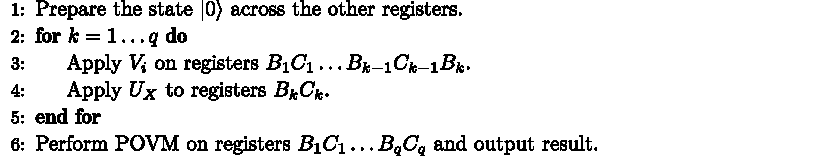
\includegraphics[width=\linewidth,height=0.78\textheight,keepaspectratio]{icalp2026-3-svg-01.pdf}\par





The final state before the POVM has dimension $(2N)^{q}$ as it can be expressed as,\par


\[\begin{gathered}
\sum_{(j_{1},\ldots,j_{q})\in[N]^{q}}a_{1,j_{1}}\ket{j_{1}}\otimes\ket{X_{j_{1}}}\otimes\ldots a_{q,j_{1},\ldots,j_{q-1},X_{j_{1}},\ldots,X_{j_{q-1}},j_{q}}\ket{j_{q}}\otimes\ket{X_{j_{q}}}.
\end{gathered}\]




This expression exists in a linear subspace that has at most $(2N)^{q}$ linearly independent basis states (defined by each $(j_{1},\ldots,j_{q})\in[N]^{q}$ and $X_{j_{i}}$). This does not change if we add ancillae or additional workspace.\par




We now invoke Holevo’s bound. Given that $|\mathrm{Im}(f_{\mathcal{A}})|=m$,
let $\mathbf{X}$ be a random variable which is uniformly distributed over the set $L=\{X_{1},\ldots,X_{m}\}$
whose outputs on applying $f_{\mathcal{A}}$ are different on each element of the set $\forall i,j\in[m]:f_{\mathcal{A}}(X_{i})=f_{\mathcal{A}}(X_{j})\implies i=j$. Let $\mathbf{Y}$ be the random variable denoting the output of $\mathcal{A}$ for which the random variable $\mathbf{X}$ is the input. If the inputs are enumerated $(X_{t})_{t\in[m]}$ and the final state on input $X_{t}$ is $\rho_{t}$, then Holevo’s bound (Lemma 17 for ensemble $(\rho_{t})_{t\in[m]}$ and distribution uniform over $[m]$) states the following,\par




\[\begin{gathered}
\displaystyle I(\mathbf{X}:\mathbf{Y}) \displaystyle\leq S\left(\sum_{t=1}^{m}\frac{1}{m}\rho_{t}\right)-\sum_{t=1}^{m}\frac{1}{m}S(\rho_{t}) \\
\displaystyle\leq S\left(\sum_{t=1}^{m}\frac{1}{m}\rho_{t}\right) \\
\displaystyle\leq\log\left(\text{dim}\left(\sum_{t=1}^{m}\frac{1}{m}\rho_{t}\right)\right) \\
\displaystyle\leq q\log(2N).
\end{gathered}\]




The second line follows as each $S(\rho_{t})$ is non-negative. The third follows by the maximum entropy of a state over dimension $d$ (Remark 15).\par




The left hand side can be bounded as follows,\par


\[\begin{gathered}
\displaystyle I(\mathbf{X}:\mathbf{Y}) \displaystyle=H(\mathbf{X})-H(\mathbf{X}|\mathbf{Y}) \\
\displaystyle=\log(m)-H(\mathbf{X}|\mathbf{Y}) \\
\displaystyle\geq\log(m)-H\left(\frac{1}{3},\frac{2}{3}\right)-\frac{1}{3}\log(m) \\
\displaystyle\geq\frac{2}{3}\log(m)-2.
\end{gathered}\]


The third line follows from Fano’s inequality (Lemma 18).\par




Therefore, $q\log(2N)\geq I(\mathbf{X}:\mathbf{Y})\geq\frac{2}{3}\log(m)-2$, which implies $m=O((2N)^{3q/2})$.
$\blacktriangleleft$\par




Now we are ready to prove Theorem 4 with a similar search-to-decision argument as in the classical case ([15, Theorem 4.1]). Note that the complexity differs from that in the classical case, as classically turning a decision problem from randomized to deterministic costs a cubic overhead in complexity ($\forall f:D(f)=O(R(f)^{3})$), whereas in the quantum setting this is quartic ($\forall f:D(f)=O(Q(f)^{4})$).\par





\par\medskip\noindent\textbf{Proof of Theorem 4 .}\par




Fix a pseudo-deterministic quantum algorithm $\mathcal{A}$ with query complexity $\mathsf{psQ}(R)$.
For every $X$, there exists a canonical output $Y_{X}$ of $\mathcal{A}$. By Lemma 19, we can encode this output in $d=O(\mathsf{psQ}(R)\log(N))$ bits.
We can then define $d$ total boolean functions $(f_{i})_{i}^{d}$, where for all $i\in[d]:f_{i}(X)=(Y_{X})_{i}$, i.e., $f_{i}$ outputs the $i$-th bit of $Y_{X}$.\par




We use the following fact relating the deterministic query complexity with the quantum query complexity of a decision problem.\par



% SOURCE-ID Thmtheorem20


\par\medskip\noindent\textbf{
\textbf{Theorem 20}\textbf{ }(Theorem 2 [2])\textbf{.}
}\par



\emph{For any total boolean function $f$, the deterministic and quantum query complexity are related as follows:}\par


\[\begin{gathered}
\mathsf{D}(f_{i})=O(\mathsf{Q}(f_{i})^{4})
\end{gathered}\]



% END-SOURCE-ID Thmtheorem20



We also note that $\mathsf{Q}(f_{i})=O(\mathsf{psQ}(R))$ for all $i\in[d]$, from which we conclude that\par


\[\begin{gathered}
\mathsf{D}(R)=O\left(\sum_{i=1}^{d}\mathsf{D}(f_{i})\right)=O(d\cdot\mathsf{psQ}(R)^{4})=O(\mathsf{psQ}({R})^{5}\log(N)).\
\end{gathered}\]


$\blacktriangleleft$\par






\par\medskip\noindent\textbf{
3.2 General pseudo-deterministic quantum query upper bound}\par




We present a general quantum pseudo-deterministic query upper bound for any problem via its randomized query complexity and verification complexity.\par




% SOURCE-ID Thmtheorem5


\par\medskip\noindent\textbf{
\textbf{Theorem 5}\textbf{.}
[Restated, see original statement.]}\par



\emph{For any search problem ${R}$ with randomized query complexity $\mathsf{R}(R)$ and verification complexity $\mathsf{V}(R)$, we have $\mathsf{psQ}(R)=O\big((\mathsf{R}(R)+\mathsf{V}(R))\cdot\sqrt{N}\big)$.}\par



% END-SOURCE-ID Thmtheorem5




Our proof is a straightforward generalization of [18, Theorem 3], which shows the \emph{completeness} of Find1 (for classical pseudo-deterministic query complexity) by building a general reduction from any problem to Find1. We observe that the same reduction also works in the quantum setting, and then combine it with the $O(\sqrt{N})$ upper bound of Find1 [20]. We present a full proof of 5 in the full version of this paper.\par






\par\medskip\noindent\textbf{
4 Query complexity separations}\par




In this section, we prove two query complexity separation results for pseudo-deterministic quantum algorithms.
In Section 4.1, we present a problem that is trivial for classical randomized algorithms but maximally hard for pseudo-deterministic quantum algorithms.
In Section 4.2, we provide a problem that is easy for both classical randomized algorithms and pseudo-deterministic quantum algorithms, but difficult for classical pseudo-deterministic algorithms.\par




\par\medskip\noindent\textbf{
4.1 A maximally hard problem for pseudo-deterministic quantum algorithms}\par




We define the Avoid One Encrypted String (AOES) problem and prove that its pseudo-deterministic quantum query complexity is $\Omega(N)$, while being completely trivial for standard randomized algorithms. We prove the separation of Theorem 1 that we restate below.\par




% SOURCE-ID Thmtheorem1


\par\medskip\noindent\textbf{
\textbf{Theorem 1}\textbf{.}
[Restated, see original statement.]}\par



\emph{There exists a search problem ${R}$ whose classical randomized complexity is $O(1)$ and whose pseudo-deterministic quantum query complexity is $\Omega(N)$.}\par



% END-SOURCE-ID Thmtheorem1




We use the ${\text{XOR}}_{N}$ problem as our building block, since ${\text{XOR}}_{N}$ is (asymptotically) maximally hard for quantum query algorithms. Here, for $a,b\in\{0,1\}:a\oplus b$ is the exclusive logical-or of the two bits, and for strings $X,Y\in\{0,1\}^{r}$, $X\bigoplus Y$ is the bitwise exclusive logical-or of the two strings. We write $\mathsf{XOR}(X)$ as the exclusive or of every bit in the string $X$.\par




Here, the input of ${\text{XOR}}_{N}$ is a string of length $N$ and the output is the ${\text{XOR}}_{N}$ of each bit of the string, we write this problem as XOR without the subscript when the length is clear from context. A quantum algorithm for XOR cannot gain \emph{any} advantage over a random guess with fewer than $N/2$ queries, as captured by the following lemma.\par



% SOURCE-ID Thmtheorem21


\par\medskip\noindent\textbf{
\textbf{Lemma 21}\textbf{ }([12, 5])\textbf{.}
}\par



\emph{Suppose $\mathcal{A}$ is a quantum algorithm for the XOR problem which has advantage over a random guess. In other words, if there exists $p,\delta\in\mathbb{R}$ such that for any $X\in\{0,1\}^{N}$,}\par


\[\begin{gathered}
\mathbb{P}[\mathcal{A}^{X}=1|(\mathsf{XOR}(X)=1)]\geq p+\delta,
\end{gathered}\]


\emph{and}\par


\[\begin{gathered}
\mathbb{P}[\mathcal{A}^{X}=1|(\mathsf{XOR}(X)=0)]\leq p.
\end{gathered}\]


\emph{Then $\mathcal{A}$ must have query complexity at least $\frac{N+1}{2}$.}\par



% END-SOURCE-ID Thmtheorem21



We now define our Avoid-One-Encrypted-String (AOES) problem.
Informally, the input of AOES uses $m$ separate XOR instances to encrypt a string $b\in\{0,1\}^{m}$, and the goal is to avoid outputting the encrypted string $b$. The intuition is that since the XOR problem is maximally hard for quantum algorithms, the string $b$ cannot be decrypted, and hence the quantum algorithm cannot avoid it.
Note that the parameter $m$ controls a trade-off between the quantum pseudo-deterministic query complexity and the classical randomized query complexity. We obtain the maximal separation by choosing $m$ to be a large constant.\par



% SOURCE-ID Thmtheorem22


\par\medskip\noindent\textbf{
\textbf{Definition 22}\textbf{ }(Avoid-One-Encrypted-String (AOES))\textbf{.}
}\par



\emph{Let $m\in\mathbb{N}$. In the ${\text{AOES}}_{m}$ problem, we are given oracle access to $m$ different strings $X_{1},\ldots,X_{m}\in\{0,1\}^{N/m}$. For each $i\in[m]$ define $b_{i}=\mathsf{XOR}(X_{i})$.}\par




\emph{The goal is to output a string $x\in\{0,1\}^{m}$ such that $x\neq b$.}\par



% END-SOURCE-ID Thmtheorem22



We write AOES without the subscript when the parameters of the problem are clear from context. We also assume that $m$ divides $N$ and otherwise we can use a standard padding argument. We begin by noting that, for small values of $m$, AOES is easy for randomized algorithms and hard for deterministic algorithms\par



% SOURCE-ID Thmtheorem23


\par\medskip\noindent\textbf{
Claim 23. 
}\par



The following holds for the complexity of ${\text{AOES}}_{m}$.\par


\begin{itemize}


\item[] 
$\blacksquare$ 


$R({\text{AOES}}_{m})=O(1)$;\par





\item[] 
$\blacksquare$ 


$D({\text{AOES}}_{m})=\Theta(N/m)$.\par





\end{itemize}



% END-SOURCE-ID Thmtheorem23



\par\medskip\noindent\textbf{
\textbf{Proof}.}\par




The first item follows by uniformly randomly sampling a string $x\in\{0,1\}^{m}$ which will be a valid solution with probability $1-1/2^{m}$. The upper bound for the second item follows by calculating $b_{1}=\mathsf{XOR}(X_{1})$ using $N/m$ queries and outputting $(1\oplus b_{1})0^{m-1}$.\par




We prove the lower bound using a standard adversary argument. Suppose there exists a deterministic algorithm $\mathcal{A}$ for AOES that takes $q=N/m-1$ deterministic queries. Whenever $\mathcal{A}$ queries a bit, we set that bit equal to $0$. After $\mathcal{A}$ outputs a solution $x\in\{0,1\}^{m}$, there is at least one bit in each string $X_{i}$ that is not queried by $\mathcal{A}$. Therefore, one can set those remaining bits such that $\mathsf{XOR}(X_{i})=x_{i}$ for all $i\in[m]$, which implies $\mathcal{A}$ is wrong.
$\vartriangleleft$\par




We show that any pseudo-deterministic quantum algorithm for AOES cannot do much better than the trivial deterministic algorithm.\par



% SOURCE-ID Thmtheorem24


\par\medskip\noindent\textbf{
\textbf{Theorem 24}\textbf{ }(psQ lower bound for AOES)\textbf{.}
}\par



\emph{Let $m\in[N]$. Any pseudo-deterministic quantum algorithm for ${\text{AOES}}_{m}$ requires $\Omega(N/m^{2})$ queries.}\par



% END-SOURCE-ID Thmtheorem24



Note that by setting $m$ in Theorem 24 to be a sufficiently large constant, we obtain Theorem 1.
We prove Theorem 24 in two steps. We first transform a zero-error quantum algorithm for AOES into a quantum algorithm for the XOR problem with some \emph{non-zero} advantage. We then replace the zero-error algorithm with a pseudo-deterministic one.\par




The following lemma demonstrates that access to a single sample from an algorithm for AOES is enough to extract non-zero information about the XOR of a string.\par



% SOURCE-ID Thmtheorem25


\par\medskip\noindent\textbf{
\textbf{Lemma 25}\textbf{.}
}\par



\emph{If there exists a zero-error quantum algorithm $\mathcal{B}$ for ${\text{AOES}}_{N,m}$ with query complexity $q$, then there exists a quantum algorithm $\mathcal{A}$ for ${\text{XOR}}_{N/m}$ which calls $\mathcal{B}$ once such that for every input $X\in\{0,1\}^{N/m}$,}\par


\[\begin{gathered}
\mathbb{P}\left[\mathcal{A}^{X}=\mathsf{XOR}(X)\right]\geq\frac{1}{2}+\frac{1}{2^{m+1}}.
\end{gathered}\]



% END-SOURCE-ID Thmtheorem25




\par\medskip\noindent\textbf{Reduction}\par




We use $\mathcal{B}$ to construct an algorithm $\mathcal{A}$ for ${\text{XOR}}_{N/m}$. In this algorithm, we encode the XOR instance $X$ into a randomized instance of ${\text{AOES}}_{m}$, which is information theoretically indistinguishable to a uniformly random instance from $\mathcal{B}$’s perspective. If $\mathcal{B}$’s output meets certain conditions, we can recover the parity of $X$ with certainty.
The pseudocode of algorithm $\mathcal{A}$ is described in Algorithm 2.\par



\textbf{Algorithm 2}  Algorithm $\mathcal{A}^{X}$ for ${\text{XOR}}_{N/m}$ induced from algorithm $\mathcal{B}$ for ${\text{AOES}}_{N,m}$.
\par\noindent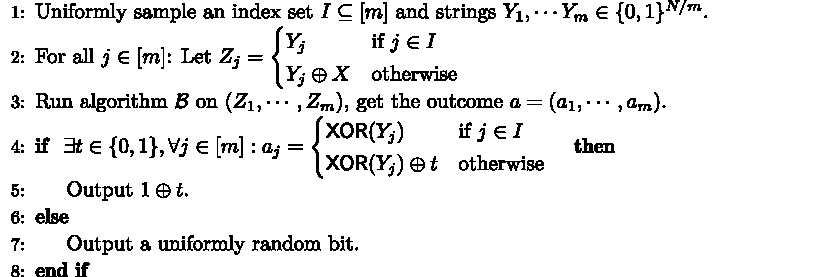
\includegraphics[width=\linewidth,height=0.78\textheight,keepaspectratio]{icalp2026-3-svg-02.pdf}\par





\par\medskip\noindent\textbf{Analysis}\par




We now show the correctness of algorithm $\mathcal{A}$.
For simplicity, we define the following bits\par


\[\begin{gathered}
\displaystyle x^{*} \displaystyle=\mathsf{XOR}(X),\,\forall j\in[m]:y_{j}=\mathsf{XOR}(Y_{j}),\,z_{j}=\mathsf{XOR}(Z_{j}).
\end{gathered}\]




After the first three steps of algorithm $\mathcal{A}$, we get $(a_{1},\cdots,a_{m})$ as a valid solution to the AOES instance $(Z_{1},\ldots,Z_{m})$. Now, we define the following set\par


\[\begin{gathered}
J\coloneqq\{j\in[m]:a_{j}=z_{j}\}.
\end{gathered}\]


Note that $\mathcal{A}$ cannot calculate $J$ directly, because $\mathcal{A}$ does not know the value of $z_{j}$ when $j\not\in I$. Nevertheless, $\mathcal{A}$ can always test whether $J$ is equal to $I$, as shown in the following claim.\par



% SOURCE-ID Thmtheorem26


\par\medskip\noindent\textbf{
Claim 26. 
}\par



The condition at Line 4 is satisfied if and only if $I=J$.\par



% END-SOURCE-ID Thmtheorem26



\par\medskip\noindent\textbf{
\textbf{Proof}.}\par




For one direction, if $I=J$, then for any $j\in[m]$, it holds that\par


\[\begin{gathered}
a_{j}=\begin{cases}z_{j}&\text{if }j\in I\\
z_{j}\oplus 1&\text{otherwise }\end{cases}.
\end{gathered}\]




Now replace $z_{j}$ with $y_{j}$ if $j\in I$, or with $(y_{j}\oplus x^{*})$ otherwise, we get\par


\[\begin{gathered}
a_{j}=\begin{cases}y_{j}&\text{if }j\in I\\
y_{j}\oplus x^{*}\oplus 1&\text{otherwise }\end{cases}.
\end{gathered}\]




Therefore, the condition at Line 5 is satisfied by taking $t=x^{*}\oplus 1$.\par




For the other direction, if the condition at Line 4 holds, we can rewrite this condition by replacing $y_{j}$ with $z_{j}$ or $(z_{j}\oplus x^{*})$ for $j\in I$ or $j\not\in I$ respectively; it holds that\par


\[\begin{gathered}
a_{j}=\begin{cases}z_{j}&\text{if }j\in I\\
z_{j}\oplus x^{*}\oplus t&\text{otherwise }\end{cases}.
\end{gathered}\]




We claim that $x^{*}\oplus t=1$; otherwise, we have $a_{j}=z_{j}$ for all $j\in[m]$, which contradicts to the fact that $a$ is a valid solution to the AOES instance. Therefore, we have $I=J$ by the definition of $J$.
$\vartriangleleft$\par




The proof of Claim 26 immediately implies the following corollary.\par



% SOURCE-ID Thmtheorem27


\par\medskip\noindent\textbf{
Claim 27. 
}\par



Algorithm $\mathcal{A}$ always outputs the correct answer at Line 5.\par



% END-SOURCE-ID Thmtheorem27




\par\medskip\noindent\textbf{
\textbf{Proof}.}\par




In the proof of Claim 26, we show that if the condition at Line 4 holds, it must be the case that $x^{*}\oplus t=1$. Thus, $x^{*}=t\oplus 1$ is the correct answer.
$\vartriangleleft$\par



% SOURCE-ID Thmtheorem28


\par\medskip\noindent\textbf{
Claim 28. 
}\par



The condition at Line 4 is satisfied with probability $1/2^{m}$.\par



% END-SOURCE-ID Thmtheorem28




\par\medskip\noindent\textbf{
\textbf{Proof}.}\par




By Claim 26, it suffices to show that $I=J$ happens with probability $1/2^{m}$.
Note that $I$ is chosen independently with $Y_{1},\ldots,Y_{m}$, and $Y_{1},\ldots,Y_{m}$ is uniformly random. Therefore, $I$ is also independent with $(Z_{1},\ldots,Z_{m})$.
Since the set $J$ only depends on $(Z_{1},\ldots,Z_{m})$ and the internal randomness of $\mathcal{B}$, $I$ and $J$ are also independent. Therefore, $I$ is equal to $J$ with probability $1/2^{m}$.
$\vartriangleleft$\par




Combining Claim 27 and Claim 28, the overall success probability of $\mathcal{A}$ is\par


\[\begin{gathered}
\frac{1}{2^{m}}+\frac{1}{2}(1-\frac{1}{2^{m}})=\frac{1}{2}+\frac{1}{2^{m+1}},
\end{gathered}\]


which concludes Lemma 25.\par




Finally, we show that we can replace the zero-error algorithm for AOES in Lemma 25 with a pseudo-deterministic algorithm with a small overhead on the query complexity.\par



% SOURCE-ID Thmtheorem29


\par\medskip\noindent\textbf{
\textbf{Lemma 29}\textbf{.}
}\par



\emph{If there exists a pseudo-deterministic quantum algorithm $\mathcal{B}$ for ${\text{AOES}}_{N,m}$ with query complexity $q$, then there exists a quantum algorithm $\mathcal{A}$ for ${\text{XOR}}_{N/m}$ with query complexity $O(q\cdot m)$ such that for every input $X\in\{0,1\}^{N/m}$,}\par


\[\begin{gathered}
\mathbb{P}\left[\mathcal{A}^{X}=\mathsf{XOR}(X)\right]\geq\frac{1}{2}+\frac{1}{2^{m+2}}.
\end{gathered}\]



% END-SOURCE-ID Thmtheorem29




\par\medskip\noindent\textbf{Proof.}\par




Given such a pseudo-deterministic algorithm $\mathcal{B}$, we can construct a new algorithm $\mathcal{B}^{\prime}$ that repeatedly runs $\mathcal{B}^{X}$ for $100m$ times and outputs the most common outcomes from these repetitions (breaking ties arbitrarily).
By the Chernoff bound, the error probability of $\mathcal{B}^{\prime}$ is smaller than $\frac{1}{2^{m+2}}$.\par




Since the zero-error algorithm for AOES is only called once in Lemma 25, we can replace it by $\mathcal{B^{\prime}}$, and only increase the overall error probability by at most $\frac{1}{2^{m+2}}$.
$\blacktriangleleft$\par




Combining Lemma 29 with Lemma 21, we conclude Theorem 24.\par



% SOURCE-ID Thmtheorem30


\par\medskip\noindent\textbf{
$\blacktriangleright$ Remark 30.
}\par



\emph{The only place we use the pseudo-deterministic property for proving Theorem 24 is the repetition trick in Lemma 29. In contrast, the trivial random sampling algorithm for AOES has error probability $1/2^{m}$; however, we cannot reduce this error via repetition.}\par




\emph{Indeed, our proof of Theorem 24 implies that achieving an error probability that is much lower than $1/{2^{m}}$ for AOES is extremely difficult, even for a standard quantum algorithm.}\par



% END-SOURCE-ID Thmtheorem30






\par\medskip\noindent\textbf{
4.2 Exponential pseudo-deterministic quantum advantage}\par




In this section, we define a problem, Quantum-Locked Estimation (QL-Estimation), which is hard for classical algorithms to solve pseudo-deterministically, but is easy for pseudo-deterministic quantum algorithms and randomized classical algorithms.\par




% SOURCE-ID Thmtheorem3


\par\medskip\noindent\textbf{
\textbf{Theorem 3}\textbf{.}
[Restated, see original statement.]}\par



\emph{There exists a search problem ${R}$ such that}\par


\begin{enumerate}


\item[] 
1. 


\emph{there exists a randomized classical algorithm }$\mathcal{A}$\emph{ for }${R}$\emph{ that uses }$O(\log N)$\emph{ queries;}\par





\item[] 
2. 


\emph{there exists a quantum pseudo-deterministic algorithm }$\mathcal{B}$\emph{ with }$O(\log N)$\emph{ query complexity that canonizes }$\mathcal{A}$\emph{;}\par





\item[] 
3. 


\emph{any classical pseudo-deterministic algorithm for }${R}$\emph{ requires }$\Omega(\sqrt{N})$\emph{ queries.}\par





\end{enumerate}



% END-SOURCE-ID Thmtheorem3




The QL-Estimation problem can be seen as
a \emph{lock-and-key} construction. We first pick the Hamming problem – calculating an estimate of the Hamming weight of a string – as the “lock”, since it is easy for classical randomized algorithms but hard for any pseudo-deterministic classical algorithm. We then add in a “key”, the Simon’s problem [22], as a search problem with exponential quantum advantage, and the unique solution of the “key” problem is a valid solution of the “lock” problem.
Combining these, the input to the lock-and-key promise problem is a pair $(f,X)$. An input of this form satisfies the promise (and is therefore a valid input) if the solution of the key problem on input $f$ is a solution to the lock problem on input $X$ and any valid solution overall is a solution to the lock problem on input $X$. This implies that a quantum algorithm can obtain the secret string that is the pseudo-deterministic solution to this problem that we know is classically pseudo-deterministically hard.\par




In this section, unless otherwise stated, $N=2^{n}$.
We start by introducing the following necessary definitions.\par



% SOURCE-ID Thmtheorem31


\par\medskip\noindent\textbf{
\textbf{Definition 31}\textbf{ }(Simon’s Problem)\textbf{.}
}\par



\emph{The input to this problem is a function $f:\{0,1\}^{n}\rightarrow\{0,1\}^{n}$ promised to be a 2-to-1 or 1-to-1 function with a secret string $s\in\{0,1\}^{n}$ such that}\par


\[\begin{gathered}
\forall x,y\in\{0,1\}^{n}:f(x)=f(y)\iff x=y\oplus s\;\text{ or }\;x=y.
\end{gathered}\]


\emph{Given oracle access to this function, the goal is to output the secret string $s$. The special case $s=0^{n}$ implies that $f$ is a permutation of the strings of length $n$.}\par



% END-SOURCE-ID Thmtheorem31



With some abuse of notation, we interpret $s\in\{0,1\}^{n}$ to be either a string or an $n$-bit binary number interchangeably. For $s\in\{0,1\}^{n}$, we denote by $\mathcal{F}_{s}$ the set of Simon’s functions on $\{0,1\}^{n}$ that encode the secret string $s$, that is all functions $f:\{0,1\}^{n}\rightarrow\{0,1\}^{n}$ such that for every distinct $x,y\in\{0,1\}^{n}$ it holds that $f(x)=f(y)$ if and only if $x=y$ or $x=y\oplus s$. We shall use the following standard bounds of the query complexity of Simon’s problem.\par



% SOURCE-ID Thmtheorem32


\par\medskip\noindent\textbf{
\textbf{Theorem 32}\textbf{ }([22])\textbf{.}
}\par



\emph{Any classical randomized algorithm for Simon’s problem requires $\Omega(2^{n/2})$ queries, whereas there exists a quantum algorithm for Simon’s problem using $O(n)$ queries.}\par



% END-SOURCE-ID Thmtheorem32



Indeed, we require the following stronger statement regarding the hardness of Simon’s problem.\par



% SOURCE-ID Thmtheorem33


\par\medskip\noindent\textbf{
\textbf{Lemma 33}\textbf{.}
}\par



\emph{Given a function $f\in\mathcal{F}_{s}$
where the secret string $s$ is promised to be in one of two disjoint sets $S_{1},S_{2}\subseteq\{0,1\}^{n}$, then any classical randomized algorithm needs $\Omega(\sqrt{\min(|S_{1}|,|S_{2}|)})$ queries to determine whether $s$ is in $S_{1}$ or $S_{2}$.}\par



% END-SOURCE-ID Thmtheorem33



\par\medskip\noindent\textbf{Proof.}\par




With half the probability, let the secret string $s$ be uniformly drawn from $S_{1}$; and with half the probability, let $s$ be uniformly drawn from $S_{2}$. Then, take $f$ to be uniformly drawn from $\mathcal{F}_{s}$.\par




By Yao’s minimax principle, it suffices to consider any deterministic algorithm $\mathcal{A}$ making at most $t=o(\sqrt{\min(|S_{1}|,|S_{2}|)})$ queries on the input distribution above. Without loss of generality, we assume $\mathcal{A}$ will stop and output the answer immediately once it finds a collision of $f$.
By symmetry, we can simplify the decision tree of $\mathcal{A}$ by merging nodes in a way that each non-leaf node has only two children: one represents that a collision is found, and the other represents that no collision is found.\par




We call a string $t$ at node $u$ \emph{alive} if the queries to $u$’s ancestors have not ruled out the possibility that the secret string of $f$ being $t$. All the strings in $S_{1}$ and $S_{2}$ are alive at the root, and a query at depth $d$ can \emph{kill} at most $d-1$ strings. By symmetry, the probability that $\mathcal{A}$ never finds a collision is $1-o(1)$. And conditioned on reaching a leaf $u$ without collision, most of the strings in both $S_{1}$ and $S_{2}$ are still alive at $u$. Thus, no matter $\mathcal{A}$ outputs $S_{1}$ or $S_{2}$ at $u$, $\mathcal{A}$ will be wrong with probability at least $\frac{1}{2}-o(1)$. This concludes that $\mathcal{A}$ is not correct, and thus $\Omega(\sqrt{\min(|S_{1}|,|S_{2}|)})$ queries are necessary.
$\blacktriangleleft$\par




We now formally state the version of the Hamming weight approximate problem that we will denote by Hamming.\par



% SOURCE-ID Thmtheorem34


\par\medskip\noindent\textbf{
\textbf{Definition 34}\textbf{ }(The Hamming Problem)\textbf{.}
}\par



\emph{Given a bit string $X\in\{0,1\}^{N}$, the goal is to output an approximation of the Hamming weight of $X$ within an additive error range of $N/10$; that is,}\par


\[\begin{gathered}
\displaystyle{\text{Hamming}}=\{(X,t)\in\{0,1\}^{N}\times\mathbb{N}:\big|\|X\|_{\mathsf{hw}}-t\big|\leq N/10\}\;.
\end{gathered}\]



% END-SOURCE-ID Thmtheorem34



Since we allow a solution to Hamming to be within a range of the actual Hamming weight, it can be easily solved by a random sampling algorithm in $O(1)$ queries.
However, Hamming was proven to be maximally hard for classical pseudo-deterministic algorithm in [15]. We reproduce the proof here, as it includes some useful ideas for proving the lower bound of the QL-Estimation problem later.\par



% SOURCE-ID Thmtheorem35


\par\medskip\noindent\textbf{
\textbf{Theorem 35}\textbf{ }(Corollary 3.2 of [15])\textbf{.}
}\par



$\mathsf{psR}({\text{Hamming}})=\Omega(N)$\emph{.}\par



% END-SOURCE-ID Thmtheorem35




\par\medskip\noindent\textbf{Proof.}\par




Now let $\mathcal{A}$ be a pseudo-deterministic algorithm for Hamming.
Let $X^{*}\in\{0,1\}^{N}$ be some fixed string whose Hamming weight is $N/2$, and take
$t\coloneqq\mathcal{A}^{X^{*}}$. We then pick a string $Y\in\{0,1\}^{N}$ whose Hamming weight is the smallest among those for which $\mathcal{A}$ outputs $t$ with probability at least $2/3$ (break ties arbitrarily).
The Hamming weight of $Y$ is at least $3N/10$.\par




Now consider the set $\mathcal{E}_{Y}$ of strings by flipping a “1” to “0” in $Y$, i.e.,\par


\[\begin{gathered}
\mathcal{E}_{Y}\coloneqq\{X\in\{0,1\}^{N}:\exists i\in[N],X_{i}=0\land Y_{i}=1\land(X_{j}=Y_{j},\forall j\neq i)\}.
\end{gathered}\]


By definition, we have $\mathcal{A}^{Y}\neq\mathcal{A}^{Y^{\prime}}$ for any string $Y^{\prime}\in\mathcal{E}_{Y}$; we also know $|\mathcal{E}_{Y}|\geq 3N/10$.
Therefore, $\mathcal{A}$ requires $\Omega(N)$ queries to distinguish $Y$ from all the strings in $\mathcal{E}_{Y}$.
$\blacktriangleleft$\par




We now state the QL-Estimation problem, where the Simon’s problem is the “key” and Hamming is the “lock”.\par



% SOURCE-ID Thmtheorem36


\par\medskip\noindent\textbf{
\textbf{Definition 36}\textbf{ }(The QL-Estimation Problem)\textbf{.}
}\par



\emph{The input is a pair $(f,X)$ for $f:\{0,1\}^{n}\rightarrow\{0,1\}^{n}$ and $X\in\{0,1\}^{N}$ where $N=2^{n}$. Here, $(f,X)$ is promised to satisfy the following.}\par


\begin{itemize}


\item[] 
$\blacksquare$ 


$f\in\mathcal{F}_{s}$\emph{ for a string }${s}\in\{0,1\}^{n}$\emph{, i.e., }$f$\emph{ is a valid Simon’s instance encoding the secret }$s$\emph{;}\par





\item[] 
$\blacksquare$ 


$\big|\|X\|_{\mathsf{hw}}-{s}\big|\leq 0.09\cdot N$\emph{, i.e., the value of }${s}$\emph{ is a valid solution to the }Hamming\emph{ instance }$X$\emph{.}\par





\end{itemize}




\emph{The goal is to output an integer $t\in[N]$ within $N/10$ distance of the Hamming weight of $X$.}\par



% END-SOURCE-ID Thmtheorem36



In this case, a query to an input $(f,X)$ of QL-Estimation is either a query to $f$ or to $X$ and the query complexity of an algorithm for QL-Estimation is the total number of queries to either part of the input. We show that QL-Estimation is easy for classical randomized and a quantum pseudo-deterministic algorithm exists that canonizes the classical one, but the problem is hard for classical pseudo-deterministic algorithm; this immediately implies Theorem 3.\par



% SOURCE-ID Thmtheorem37


\par\medskip\noindent\textbf{
\textbf{Theorem 37}\textbf{.}
}\par



\emph{Let $N=2^{n}$ be the length parameter in QL-Estimation, then the following holds for the complexity of QL-Estimation.}\par


\begin{enumerate}


\item[] 
1. 


$\mathsf{R}({\text{QL-Estimation}})=O(1)$\emph{;}\par





\item[] 
2. 


$\mathsf{psQ}({\text{QL-Estimation}})=O(\log N)$\emph{;}\par





\item[] 
3. 


$\mathsf{psR}({\text{QL-Estimation}})=\Omega(\sqrt{N})$\emph{.}\par





\end{enumerate}


\emph{Furthermore, there exists a classical randomized algorithm $\mathcal{A}$ for QL-Estimation with query complexity $O(\log N)$ and a pseudo-deterministic quantum algorithm $\mathcal{B}$ with query complexity $O(\log(N))$ such that $\mathcal{B}$ canonizes $\mathcal{A}$.}\par



% END-SOURCE-ID Thmtheorem37




\par\medskip\noindent\textbf{Upper bounds and canonization}\par




The first upper bound follows as a classical randomized algorithm can solve the Hamming part directly via sampling and ignore the Simon’s problem with $O(1)$ queries via random sampling. For the second upper bound, note that a pseudo-deterministic quantum algorithm can also solve QL-Estimation using $O(\log N)$ queries by first solving for the secret string $s$ given $f$ in the Simon’s problem, and then outputting ${s}$ as the estimate of the Hamming weight.\par




For the last remark on canonization (Definition 2), we take the quantum algorithm $\mathcal{B}$ to be one that solves and outputs the secret string $s$ as described above.
However, we need to construct a modified randomized algorithm $\mathcal{A}$, described in below:\par


\begin{enumerate}


\item[] 
1. 


Make $10^{6}\cdot\log N$ queries to $X$ and let $\hat{t}$ be its best estimation of the Hamming weight of $X$.\par





\item[] 
2. 


Output a uniformly random integer in the range $I\coloneqq[\hat{t}-0.095N,\hat{t}+0.095N]$.\par





\end{enumerate}




By the Chernoff bound, the probability that $\big|\hat{t}-\|X\|_{\mathsf{hw}}\big|\leq 0.005N$ is $\big(1-o(1/N)\big)$. In that case, $\mathcal{A}$ always outputs a correct solution, and we have $s\in I$ by the promise of the QL-Estimation problem.
Thus, the canonical output $s$ of $\mathcal{B}$ will be outputted by $\mathcal{A}$ with probability $\Omega(1/N)$. This concludes that $\mathcal{B}$ canonizes $\mathcal{A}$\par





\par\medskip\noindent\textbf{Pseudo-deterministic lower bound}\par




To show the $\Omega(\sqrt{N})$ lower bound for any classical pseudo-deterministic algorithm, we claim that any sub-linear pseudo-deterministic classical algorithm for QL-Estimation must \emph{approximately} solve the underlying Simon’s problem, implying a lower bound from the classical hardness of Simon’s.\par



% SOURCE-ID Thmtheorem38


\par\medskip\noindent\textbf{
\textbf{Lemma 38}\textbf{.}
}\par



\emph{Let $\mathcal{A}$ be a pseudo-deterministic classical algorithm for QL-Estimation that uses $o(N)$ queries. For any string $X^{*}\in\{0,1\}^{N}$ such that $\|X^{*}\|_{\mathsf{hw}}=N/2$ and any string $s\in\{0,1\}^{n}$ whose value is between $0.41N$ and $0.59N$, it holds that for any Simon’s function $f\in\mathcal{F}_{s}$, the canonical output of $\mathcal{A}$ on input $(f,X^{*})$ is some $t$ for which $|s-t|\leq 0.01N$.}\par



% END-SOURCE-ID Thmtheorem38



\par\medskip\noindent\textbf{Proof.}\par




Take $\mathcal{A},X^{*},s$ as objects that satisfy the conditions in the statement of Lemma 38 and consider an arbitrary $f\in\mathcal{F}_{s}$ and let $t$ be the canonical output of $\mathcal{A}$ on input $(f,X^{*})$. By the correctness of $\mathcal{A}$, we have $2N/5\leq t\leq 3N/5$.\par




We then pick a string $Y_{\mathsf{low}}$ whose Hamming weight is the smallest given that $\mathcal{A}^{(f,\cdot)}$ outputs $t$ (break ties arbitrarily). The Hamming weight of $Y_{\mathsf{low}}$ is at least $2N/5-N/10=3N/10$. We claim that $\|Y_{\mathsf{low}}\|_{\mathsf{hw}}=s-0.09N$.\par




Suppose otherwise, i.e., $\|Y_{\mathsf{low}}\|_{\mathsf{hw}}>s-0.09N$, we define the set $\mathcal{E}_{\mathsf{low}}$ of strings reached by flipping any “1” to a “0” in $Y_{\mathsf{low}}$. For any string $Y^{\prime}\in\mathcal{E}_{\mathsf{low}}$, we have $\|Y^{\prime}\|_{\mathsf{hw}}\geq s-0.09N$, so $(f,Y^{\prime})$ is a valid input to the QL-Estimation problem.
Recall that $t$ is the canonical output of $\mathcal{A}$ on input $(f,Y_{\mathsf{low}})$ and let $t^{\prime}$ be the canonical output of $\mathcal{A}$ on input $(f,Y^{\prime})$. By definition of $Y_{\mathsf{low}}$, we have that $t\neq t^{\prime}$. We know $|\mathcal{E}_{\mathsf{low}}|\geq 3N/10$, which means $\mathcal{A}$ needs at least $\Omega(N)$ queries to distinguish $Y_{\mathsf{low}}$ with all the strings in $\mathcal{E}_{\mathsf{low}}$. This contradicts the assumption that $\mathcal{A}$ uses $o(N)$ queries. Thus, we conclude that $\|Y_{\mathsf{low}}\|_{\mathsf{hw}}=s-0.09N$.\par




Similarly, we can take $Y_{\mathsf{hi}}$ to be the string with largest Hamming weight such that $\mathcal{A}^{(f,\cdot)}$ outputs $t$. By symmetry, we have $\|Y_{\mathsf{hi}}\|_{\mathsf{hw}}=s+0.09N$. Since $t$ is a valid solution for both $Y_{\mathsf{hi}}$ and $Y_{\mathsf{low}}$, we have that $|t-(s-0.09N)|\leq N/10$ and $|t-(s+0.09N)|\leq N/10$. This implies $|s-t|\leq 0.01N$.
$\blacktriangleleft$\par




Now we are ready to prove the lower bound for classical pseudo-deterministic algorithms.\par





\par\medskip\noindent\textbf{Proof of Theorem 37, Item 3.}\par




Define the sets\par


\[\begin{gathered}
S_{1}=\{s:0.4N\leq s\leq 0.45N\},\;S_{2}=\{s:0.55N\leq s\leq 0.6N\}.
\end{gathered}\]


We know $|S_{1}|=|S_{2}|=N/20=\Omega(N)$.\par




Suppose the secret string $s$ is promised to be in one of $S_{1},S_{2}$ and the goal is to distinguish between these two cases, Lemma 33 shows that the randomized query complexity of this task is still $\Omega(\sqrt{N})$.\par




Now, let $\mathcal{A}$ be any classical pseudo-deterministic algorithm for QL-Estimation with $o(N)$ query complexity. If given a Simon’s function $f\in\mathcal{F}_{s}$ such that $s$ is in $S_{1}$ or $S_{2}$, we can run $\mathcal{A}^{(f,X^{*})}$ for some $X^{*}$ with $\|X^{*}\|_{\mathsf{hw}}=N/2$, and take $t$ to be its pseudo-deterministic solution. By Lemma 38, we must have $t\leq 0.46N$ or $t\geq 0.54N$, which allow us to determine whether $s\in S_{1}$ or $s\in S_{2}$. Therefore, the query complexity of $\mathcal{A}$ is $\Omega(\sqrt{N})$.
$\blacktriangleleft$\par








\par\medskip\noindent\textbf{References}\par



\begin{itemize}


\item[] 
[1]

Scott Aaronson.


BQP and the polynomial hierarchy.


In Leonard J. Schulman, editor, \emph{Proceedings of the 42nd ACM
Symposium on Theory of Computing, STOC 2010, Cambridge, Massachusetts, USA,
5-8 June 2010}, pages 141–150. ACM, 2010.


doi:10.1145/1806689.1806711.





\item[] 
[2]

Scott Aaronson, Shalev Ben-David, Robin Kothari, Shravas Rao, and Avishay
Tal.


Degree vs. approximate degree and quantum implications of huang’s
sensitivity theorem.


In Samir Khuller and Virginia Vassilevska Williams, editors, \emph{STOC ’21: 53rd Annual ACM SIGACT Symposium on Theory of Computing,
Virtual Event, Italy, June 21-25, 2021}, pages 1330–1342. ACM, 2021.


doi:10.1145/3406325.3451047.





\item[] 
[3]

Scott Aaronson and Shih-Han Hung.


Certified randomness from quantum supremacy.


In Barna Saha and Rocco A. Servedio, editors, \emph{Proceedings of the
55th Annual ACM Symposium on Theory of Computing, STOC 2023, Orlando, FL,
USA, June 20-23, 2023}, pages 933–944. ACM, 2023.


doi:10.1145/3564246.3585145.





\item[] 
[4]

Roozbeh Bassirian, Adam Bouland, Bill Fefferman, Sam Gunn, and Avishay Tal.


On certified randomness from fourier sampling or random circuit
sampling.


\emph{arXiv preprint}, 2021.


arXiv:2111.14846.





\item[] 
[5]

Robert Beals, Harry Buhrman, Richard Cleve, Michele Mosca, and Ronald de Wolf.


Quantum lower bounds by polynomials.


\emph{J. ACM}, 48(4):778–797, 2001.


doi:10.1145/502090.502097.





\item[] 
[6]

Vladimir Braverman, Robert Krauthgamer, Aditya Krishnan, and Shay Sapir.


Lower bounds for pseudo-deterministic counting in a stream.


In Kousha Etessami, Uriel Feige, and Gabriele Puppis, editors, \emph{50th International Colloquium on Automata, Languages, and Programming,
ICALP 2023, July 10-14, 2023, Paderborn, Germany}, volume 261 of \emph{LIPIcs}, pages 30:1–30:14. Schloss Dagstuhl – Leibniz-Zentrum für
Informatik, 2023.


doi:10.4230/LIPIcs.ICALP.2023.30.





\item[] 
[7]

Arkadev Chattopadhyay, Yogesh Dahiya, and Meena Mahajan.


Query complexity of search problems.


\emph{Electron. Colloquium Comput. Complex.}, TR23-039, 2023.


URL: https://eccc.weizmann.ac.il/report/2023/039.





\item[] 
[8]

Lijie Chen, Zhenjian Lu, Igor C. Oliveira, Hanlin Ren, and Rahul Santhanam.


Polynomial-time pseudodeterministic construction of primes.


In \emph{64th IEEE Annual Symposium on Foundations of Computer
Science, FOCS 2023, Santa Cruz, CA, USA, November 6-9, 2023}, pages
1261–1270. IEEE, 2023.


doi:10.1109/FOCS57990.2023.00074.





\item[] 
[9]

Andrew M. Childs and Jason M. Eisenberg.


Quantum algorithms for subset finding.


\emph{Quantum Inf. Comput.}, 5(7):593–604, 2005.


doi:10.26421/QIC5.7-7.





\item[] 
[10]

Peter Dixon, Aduri Pavan, and N. V. Vinodchandran.


Promise problems meet pseudodeterminism.


\emph{CoRR}, abs/2103.08589, 2021.


arXiv:2103.08589.





\item[] 
[11]

Peter Dixon, Aduri Pavan, Jason Vander Woude, and N. V. Vinodchandran.


Pseudodeterminism: promises and lowerbounds.


In Stefano Leonardi and Anupam Gupta, editors, \emph{STOC ’22: 54th
Annual ACM SIGACT Symposium on Theory of Computing, Rome, Italy, June 20
- 24, 2022}, pages 1552–1565. ACM, 2022.


doi:10.1145/3519935.3520043.





\item[] 
[12]

Edward Farhi, Jeffrey Goldstone, Sam Gutmann, and Michael Sipser.


Limit on the speed of quantum computation in determining parity.


\emph{Physical Review Letters}, 81(24):5442, 1998.





\item[] 
[13]

Eran Gat and Shafi Goldwasser.


Probabilistic search algorithms with unique answers and their
cryptographic applications.


\emph{Electron. Colloquium Comput. Complex.}, TR11-136, 2011.


URL: https://eccc.weizmann.ac.il/report/2011/136.





\item[] 
[14]

Michel X. Goemans, Shafi Goldwasser, and Dhiraj Holden.


Doubly-efficient pseudo-deterministic proofs.


\emph{CoRR}, abs/1910.00994, 2019.


arXiv:1910.00994.





\item[] 
[15]

Oded Goldreich, Shafi Goldwasser, and Dana Ron.


On the possibilities and limitations of pseudodeterministic
algorithms.


In Robert D. Kleinberg, editor, \emph{Innovations in Theoretical
Computer Science, ITCS ’13, Berkeley, CA, USA, January 9-12, 2013}, pages
127–138. ACM, 2013.


doi:10.1145/2422436.2422453.





\item[] 
[16]

Shafi Goldwasser, Ofer Grossman, and Dhiraj Holden.


Pseudo-deterministic proofs.


In Anna R. Karlin, editor, \emph{9th Innovations in Theoretical
Computer Science Conference, ITCS 2018, January 11-14, 2018, Cambridge, MA,
USA}, volume 94 of \emph{LIPIcs}, pages 17:1–17:18. Schloss Dagstuhl –
Leibniz-Zentrum für Informatik, 2018.


doi:10.4230/LIPIcs.ITCS.2018.17.





\item[] 
[17]

Shafi Goldwasser, Ofer Grossman, Sidhanth Mohanty, and David P. Woodruff.


Pseudo-deterministic streaming.


In Thomas Vidick, editor, \emph{11th Innovations in Theoretical
Computer Science Conference, ITCS 2020, January 12-14, 2020, Seattle,
Washington, USA}, volume 151 of \emph{LIPIcs}, pages 79:1–79:25. Schloss
Dagstuhl – Leibniz-Zentrum für Informatik,
2020.


doi:10.4230/LIPIcs.ITCS.2020.79.





\item[] 
[18]

Shafi Goldwasser, Russell Impagliazzo, Toniann Pitassi, and Rahul Santhanam.


On the pseudo-deterministic query complexity of NP search problems.


In Valentine Kabanets, editor, \emph{36th Computational Complexity
Conference, CCC 2021, July 20-23, 2021, Toronto, Ontario, Canada (Virtual
Conference)}, volume 200 of \emph{LIPIcs}, pages 36:1–36:22. Schloss Dagstuhl
– Leibniz-Zentrum für Informatik, 2021.


doi:10.4230/LIPIcs.CCC.2021.36.





\item[] 
[19]

Ofer Grossman, Meghal Gupta, and Mark Sellke.


Tight space lower bound for pseudo-deterministic approximate
counting.


In \emph{64th IEEE Annual Symposium on Foundations of Computer
Science, FOCS 2023, Santa Cruz, CA, USA, November 6-9, 2023}, pages
1496–1504. IEEE, 2023.


doi:10.1109/FOCS57990.2023.00091.





\item[] 
[20]

Robin Kothari.


An optimal quantum algorithm for the oracle identification problem.


In Ernst W. Mayr and Natacha Portier, editors, \emph{31st
International Symposium on Theoretical Aspects of Computer Science, STACS
2014, Lyon, France, March 5-8, 2014}, LIPIcs, pages 482–493. Schloss
Dagstuhl – Leibniz-Zentrum für Informatik, 2014.


doi:10.4230/LIPIcs.STACS.2014.482.





\item[] 
[21]

Michael A. Nielsen and Isaac L. Chuang.


\emph{Quantum Computation and Quantum Information (10th Anniversary
edition)}.


Cambridge University Press, 2016.


URL:
https://www.cambridge.org/de/academic/subjects/physics/quantum-physics-quantum-information-and-quantum-computation/quantum-computation-and-quantum-information-10th-anniversary-edition?format=HB.





\item[] 
[22]

Daniel R. Simon.


On the power of quantum computation.


\emph{SIAM J. Comput.}, 26(5):1474–1483, 1997.


doi:10.1137/S0097539796298637.





\item[] 
[23]

Takashi Yamakawa and Mark Zhandry.


Verifiable quantum advantage without structure.


\emph{J. ACM}, 71(3):20, 2024.


doi:10.1145/3658665.





\end{itemize}


\end{document}
